\documentclass[conference, letterpaper]{IEEEtran}

\widowpenalty 10000
\clubpenalty 10000

\usepackage{amsmath}
\usepackage{tikz}
\usepackage{pgf}
\usepackage{algorithm}
\usepackage{algpseudocode}
\usepackage{comment}


% The following can be removed in camera-ready version
\usepackage{soul} 
\renewcommand{\hl}[1]{{\leavevmode\color{red}{#1}}}



\hyphenation{op-tical net-works semi-conduc-tor}    

\usetikzlibrary{arrows,automata,arrows.meta, shapes}

\begin{document}

\title{Vegvisir: A Partition-Tolerant Blockchain \\ for the Internet-of-Things}
%\titlenote{Title is a work in progress}

\author{\IEEEauthorblockN{Kolbeinn Karlsson, Weitao Jiang\\ Stephen Wicker}
\IEEEauthorblockA{School of Electrical and Computer Engineering\\
Cornell University\\
Ithaca, New York \\
e-mail: \{kk752, wj236, sbw11\}@cornell.edu}
\and
\IEEEauthorblockN{Danny Adams, Edwin Ma\\ Robbert van Renesse, Hakim Weatherspoon}
\IEEEauthorblockA{Department of Computer Science\\
Cornell University
\\ Ithaca, New York\\
e-mail: \{da469, em577\}@cornell.edu, \{rvr,hweather\}@cs.cornell.edu
}}

\maketitle

\begin{abstract}
While the intersection of blockchains and the Internet of Things (IoT) have received considerable research interest lately, Nakamoto-style blockchains possess a number of qualities that make them poorly suited for many IoT scenarios. Specifically, they require high network connectivity and are power-intensive. This is a drawback in IoT environments where battery-constrained nodes form an unreliable ad hoc network such as in digital agriculture. In this paper we present Vegvisir, a partition-tolerant blockchain for use in power-constrained IoT environments with limited network connectivity. It is a permissioned, directed acyclic graph (DAG)-structured blockchain that can be used to create a shared, tamperproof data repository that keeps track of data provenance. We discuss the use cases, architecture, and challenges of such a blockchain.
\end{abstract}

\begin{IEEEkeywords}
blockchain, CRDT, tamper-proof logging, ad hoc networks, IoT, gossip protocols
\end{IEEEkeywords}

\section{Introduction}

Blockchains have emerged as an exciting new paradigm for distributed systems. From Bitcoin's cryptocurrency ~\cite{nakamoto_bitcoin:_2008} to Ethereum's Turing-complete smart contracts \cite{wood_ethereum:_2017}, blockchains are being explored as a means to solve problems across a wide range of industries, including banking, energy, transportation and accounting. Blockchains could have important uses in IoT and Edge Cloud environments as well \cite{christidis2016blockchains}.  Such systems are often used for applications that require tamperproof logging of events for accountability.  They are deployed under varied administrative domains, and so the decentralized ownership of blockchains make them a good match.  However, current blockchain designs require high network connectivity and are power-intensive, both of which can detract from their utility in such environments.

A blockchain is simply a tamperproof log of transactions.  Blockchain implementations use a distributed trust model, removing the need for centralized control and single-point-of-failure designs. As long as a large enough fraction of participants execute the protocol (usually half or one-third), its security properties will be enforced. This provides a system that is both  strongly consistent and highly available. It is not, however, tolerant of network partitions. Partitions cause branches (AKA forks) in the blockchain and branches must be resolved, meaning only one branch gets to stay a part of the blockchain while all others are discarded. With network partitions, such branches may stay around for a long time and lead to undesirable behaviors, even if branches are eventually resolved.  For example, people who have conducted business with Bitcoin may find that the bitcoins they were paid are now back in the hands of the original owner or have been spent otherwise.
Additionally, most current blockchain designs are very energy-intensive, requiring vast amounts of computation solving cryptopuzzles. Bitcoin alone is estimated to use tens of terawatt hours per year, enough to power a mid-sized country \cite{o2014bitcoin, beall_bitcoin_2017}. 

These two characteristics, the need for high network reliability and high power consumption, make Bitcoin and most other existing blockchain designs unsuitable for deployment in ad hoc IoT networks or edge cloud systems.  We present \emph{Vegvisir}, a blockchain specifically designed for the low-connectivity, low-power IoT setting. It tolerates network partitions well and uses a low-power consensus mechanism. Instead of resolving branches, it permits them, resulting in a Directed Acyclic Graph (DAG) structure of the blockchain rather than a linear one. The cost of this partition tolerance is that the types of applications that can be implemented with the blockchain are limited to ones that only require a partial ordering of logged events. To this end, Vegvisir supports applications based on Conflict-free Replicated Data Types (CRDT)~\cite{syn:rep:sh143}.

%The consensus mechanism, which we call Proof-of-Distribution (PoD), requires one to prove that the block has been distributed to $k$ peers other than the originator of the block. This means that $k+1$ peers claim to have stored the block, guaranteeing that if $k$ or fewer peers are malicious, the block will not be lost.  To further strengthen resilience over time, correct peers opportunistically gossip blocks with other peers they can reach.

To motivate the need for Vegvisir, we present three use cases in Section~\ref{sec:motive}. We go on to survey related literature in Section~\ref{sec:relatedworks} and develop the architecture of the blockchain in Section~\ref{sec:architecture}. Section~\ref{sec:implementation} describes our initial implementation of the blockchain and Section~\ref{sec:discussion} discusses the implications and challenges of this line of research.

\section{Motivation}\label{sec:motive}

The blockchain became popular in the financial technology sector.  However, it is generally believed that the blockchain may have far-reaching consequences for many other industries.  But many industries require interaction with the physical environment, which---unlike the fintech industry---is not always well-connected.  Below we give three examples.

\subsection{Disaster Response}
\label{sec:use-based}

The 2017 Atlantic hurricane season was one of the worst on record. Three major hurricanes devastated the Caribbean, Florida, and Texas. Hundreds of people lost their lives and the property damage is estimated to be over \$300 billion~\cite{cnn_hurricane_2017}. The loss of lives, limbs, and property had undoubtedly been greater if not for the valiant efforts of thousands of emergency first responders. If first responders could leverage more information and communication technology to aid and coordinate their efforts, further lives could potentially be saved. In an ideal world, first responders have a strong communication network and a robust cloud infrastructure that enables information to flow to the right places at the right time and eases coordination of rescue efforts. Natural disasters, however, can render communication infrastructure such as cell towers and Land Mobile Radio System (LMRS) repeaters inoperable. First responders must in those cases deploy their own communication infrastructure as well as take advantage of every possible means of communicating, forming heterogeneous ad hoc mobile networks to make up for lack of connectivity. Existing communication and cloud infrastructure is not built to operate in such environments. We need a new infrastructure design to enable first responder applications.

While cellular phones may also end up inoperable after extended periods of time in a disaster area, it is important to maximize the use of resources as long as they are available. To that end, device-to-device (D2D) communication for public safety scenarios in LTE and 5G networks has received considerable attention (see for example \cite{fodor2014device, usman2015software, doumi2013lte, yaacoub2012energy}). Our work builds on such efforts and provides distributed applications implemented on top of unreliable, ad hoc networks such as the D2D networks mentioned above.

One of the problems medical personnel face both in and outside of emergency situations is the need for accessing electronic health records promptly while safeguarding their security and privacy. We propose that blockchains can be used to implement a use-based privacy solution that gives emergency first responders ready access to sensitive patient health records but enforces strict accountability. Use-based privacy is an approach to privacy that focuses on uses (and abuses) of sensitive records, rather than access~\cite{cate_principles_2002} and has in recent years been proposed as a framework under which to design privacy policies \cite{cate_data_2013,birrell_reactive_2017}.  Patients generally will not object to a physician or paramedic accessing their medical records in order to help save their lives (a valid use) but they would object to the same physician accessing their records without a medical reason. During emergencies, paramedics and physicians could have all their access requests to sensitive records granted under the condition that the request has been recorded in a tamperproof log. Once the state of emergency is over, the log is reviewed. If frivolous access has occurred, such as a medical worker accessing an ex-spouse's or a celebrity's health record, the worker could be sanctioned, providing incentive to only access health records when necessary.

Our approach with Vegvisir presents a good avenue to implement a tamperproof log in such an environment. It consists of an unreliable network between many low-power IoT devices (first responder smartphones), some of whom cannot be fully trusted. Our solution can ensure that no health record is accessed without an explicit request for access being persistently stored on the blockchain.  It does not require proof-of-work and is therefore easy on the batteries, and its opportunistic gossip-style protocol for spreading blocks is well-suited for a mobile ad hoc network.

\subsection{Digital Agriculture}

The blockchain is a promising technology that could bring transparency and accountability to the food supply chain.  There are many participants in the food supply chain, including farmers, brokers, packers, traders, distributors, food processors, retailers, regulators, and ultimately, consumers.  Today, record keeping is mostly on paper and various centralized databases, while many negotiations are purely verbal.  This is prone to mistakes and simplifies fraud.  Farmers do not know how much profit is made on the food they supply, and consumers cannot easily track where their food comes from.  Blockchains could potentially create a shared and tamperproof data repository in which all information is readily shared, available, and auditable.

Blockchains could make it straightforward for a consumer to check the source of a food product.  In the case of a meat product, information of interest might include the animal's date of birth, place of origin, vaccinations, and use of antibiotics.  Food safety is a related application.  For example, Walmart (which sells 20\% of all food in the U.S.), IBM, and Tsinghua University are looking into using the Hyperledger blockchain \cite{cachin2016architecture} for food supply chain traceability and authenticity.  Today, if a pathogen is found in a food product, it takes several days to weeks to trace it back to the supplier. Using a blockchain, Walmart hopes to reduce this to seconds, potentially saving lives. From the farmer's perspective, blockchains could make it easier to find consumers for their products, potentially reducing waste from either unused land (if too little is produced) or from overproduction.  Farmers could check to see what retailers sell their products for, so they may negotiate a better price for their produce.

Ideally, recordkeeping with the blockchain would reach all the way to the farm and to the distribution channels.  Tagging of animals, pallets, shipping containers, and so on with RFIDs or related technology enable tracking.  But farms and distribution centers, let alone sensors, autonomous vehicles, and drones operating out in the field, have intermittent if any connection to the Internet, and must rely on a system consisting of small fixed and mobile IoT devices for sensing. While such systems can be used to create a sensor network, there is no integrated blockchain that can securely store the history of sensed data.  Again, Vegvisir allows deploying a low-energy tamperproof log in this environment.

\subsection{Maritime Industry}

According to the National Oceanic and Atmospheric Administration, the U.S. maritime transportation infrastructure was responsible for carrying  \$1.5 trillion in cargo in 2017 \cite{us_department_of_commerce}. An individual ship can hold a fortune in terms of technology, crew, and data.  The loss of a single ship could be devastating to a company's future. 

% While it is quite common for a vessel to be lost at sea, the data concerning the loss is not.
The information contained within ship systems can present valuable insight that can prevent future mishaps and save lives~\cite{howgego2018peril}. Ships can sink in solitude within a matter of minutes making it dangerous and impractical to attempt data collection under these circumstances. Moreover, retrieval of data from sunken vessels can take months to obtain and physical information from these events are sometimes unavailable due to contamination, water depth, or miscellaneous damage to instrumentation. 

Vegvisir's structure can allow for data collection on trade ships during capsizing events. Distress signals already sent out during ship emergencies could trigger the construction of an ad hoc network used by select systems on the vessel. IoT devices on lifeboats could autonomously join the network at the time of their inflation.
% We refer to systems contributing to the blockchain on the emergency WiFi as a node. 

As new nodes emerge on the network, Vegvisir's opportunistic gossip protocol can commence.
\begin{comment}
Nodes share information at specific rate with their assigned neighbors. By configuring vessel-side nodes to only gossip information with nodes on life boats, this raises the probability that all system information will be distributed amongst the life boats making it much easier to recover.
Leveraging CRDTs,
\end{comment}
Vegvisir creates a low-power consumption structure for its blockchain. This ensures that even as IoT devices acquire different information from various sources, minimal energy is spent on blockchain reconciliation. In the event of a submersion, the lifeboat nodes would still be able to gossip amongst themselves.
% eventually creating a consistent blockchain. 

Due to the nature of proprietary information in the maritime industry, Vegvisir security guarantees would be amenable in these environments. First, the secure membership protocol prevents non-verified members from contributing events. Additionally, all blocks are signed by the contributing member. Therefore, blockchain data consists only of data from approved sources regardless of network activity.
Second, Vegvisir allows for full encryption of contents within the blockchain.
\begin{comment}
By providing a stable interface for data communication, the internal contents of a blockchain are tunable to a vessel's needs. Consequently, the deployment of a company's unique encryption scheme can be performed to all field data without any major changes to the interface.
\end{comment}
These policies in conjunction serve as safeguards for company proprietary information sent over its ad hoc network while maintaining its properties of possessing tamperproof logs and being energy-efficient. 

\begin{figure*}
\centering
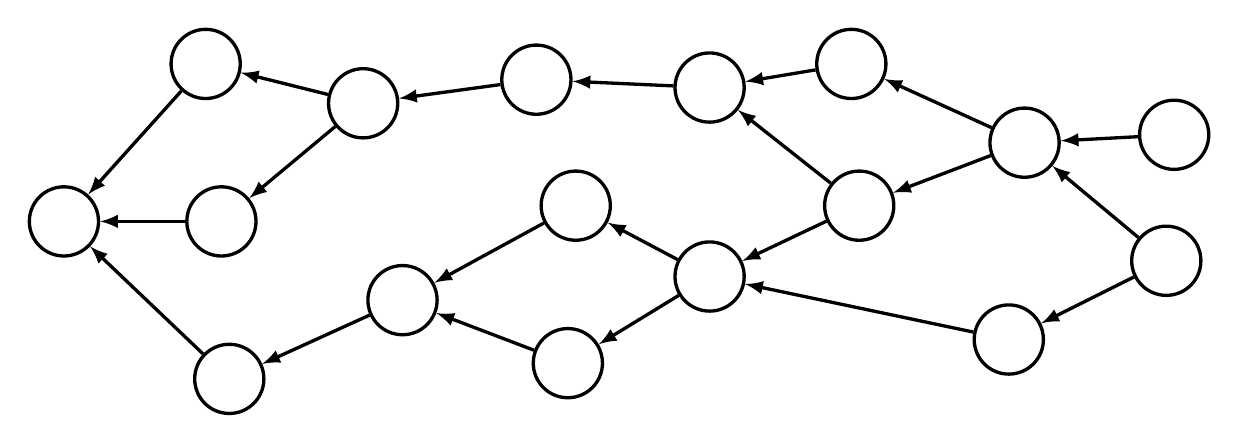
\begin{tikzpicture}[->,>=latex,auto,node distance=2.8cm,very thick]
  \tikzstyle{every state}=[fill=white,draw=black,text=black,very thick]

  \node[state] at ( 0.0, 0.0) (A) {};
  \node[state] at ( 1.8, 2.0) (B) {};
  \node[state] at ( 2.0, 0.0) (C) {};
  \node[state] at ( 2.1,-2.0) (D) {};
  \node[state] at ( 3.8, 1.5) (E) {};
  \node[state] at ( 4.3,-1.0) (F) {};
  \node[state] at ( 6.0, 1.8) (G) {};
  \node[state] at ( 6.5, 0.2) (H) {};
  \node[state] at ( 6.4,-1.8) (I) {};
  \node[state] at ( 8.2, 1.7) (J) {};
  \node[state] at ( 8.2,-0.7) (K) {};
  \node[state] at (10.0, 2.0) (L) {};
  \node[state] at (10.1, 0.2) (M) {};
  \node[state] at (12.0,-1.5) (N) {};
  \node[state] at (12.2, 1.0) (O) {};
  \node[state] at (14.0,-0.5) (P) {};
  \node[state] at (14.1, 1.1) (Q) {};

  \path (B) edge (A)
        (C) edge (A)
        (D) edge (A)
        (E) edge (B)
        (E) edge (C)        
        (F) edge (D)
        (G) edge (E)
        (H) edge (F)
        (I) edge (F)
        (J) edge (G)
        (K) edge (H)
        (K) edge (I)
        (L) edge (J)
        (M) edge (J)
        (M) edge (K)
        (O) edge (L)
        (O) edge (M)
        (N) edge (K)
        (P) edge (O)
        (P) edge (N)
        (Q) edge (O);
\end{tikzpicture}

\caption{Sample DAG. Branches are reined in by making every known leaf a predecessor of your new block. As our applications are based on CRDTs, there is no need to determine a total order between the blocks.}
\label{fig:sampledag}
\end{figure*}


\section{Related Works}
\label{sec:relatedworks}

Blockchains were first introduced in 2008 as part of the then novel Bitcoin cryptocurrency system \cite{nakamoto_bitcoin:_2008}. Since then, the blockchain field has seen explosive growth with many variants and use cases proposed. One of the more notable variants is Ethereum, which replaces the basic scripting language implemented in Bitcoin with a Turing-complete one, paving the way for so-called smart contracts \cite{wood_ethereum:_2017}. Both of these blockchains have a linear structure and rely on a proof-of-work consensus mechanism which requires solving a computationally expensive cryptopuzzle, making them poorly suited to our use cases.

Many variants on the Bitcoin protocol have been proposed since then, some of which use a DAG structure like Vegvisir. The GHOST protocol is a modification to the Bitcoin blockchain that uses a DAG structure to improve security \cite{sompolinsky_secure_2015}. The point of this modification is to enable a more robust method of selecting which fork to keep and which to discard. By keeping track of all forks, a node can choose a fork based on the heaviest-subtree-wins rule (the subtree with the largest number of blocks) as opposed to the longest-chain-wins rule, wasting less work and thus eliminating certain forms of attacks. 

The Byteball blockchain platform proposes a new type of cryptocurrency with a DAG structure \cite{churyumov_byteball:_2015}. Byteball eliminates the distinction between blocks and transactions. Each 'block' is a single transaction and can have multiple parents. Double spending is prevented by determining a total order on the DAG through the behavior of a set of privileged users called 'witnesses'. The total order is used to determine which transactions to keep and which to declare invalid when double spending occurs. 

Iota is perhaps the best-known implementation of a blockchain with a DAG structure \cite{popov_tangle_2017}. Iota is a transaction fee-less cryptocurrency where double spends are resolved by a consensus algorithm that determines which transaction to keep based on the number of descendant transactions. 

The recently proposed SPECTRE \cite{sompolinsky2016spectre} and MeshCash \cite{bentov2017tortoise} blockchains also use a DAG structure along with a protocol to reach consensus in the case of conflicts. Both are blockchains based on proof-of-work, which eliminates them from consideration for our use cases. SPECTRE's successor, PHANTOM \cite{sompolinskyphantom} requires strong network connectivity between honest nodes. HashGraph \cite{baird2016swirlds} does not rely on proof-of-work, but still requires strong network connectivity between members. 

The DAG structure in the aforementioned blockchains is not designed to provide partition tolerance like our case, but rather to exploit available parallelism for increased throughput of transactions by only ordering transactions that are dependent. As such, these blockchains expect strong network connectivity and are therefore unsuitable in our use cases.

Aside from blockchains, there are a number of non-blockchain distributed systems related to ours. Bayou, a distributed storage system for low-power mobile devices with poor network connectivity is probably one of the closest works to ours \cite{terry1995managing}. Similarly, the COPS key-value store provides causal consistency in wide-area networks \cite{lloyd_dont_2011}. Both Bayou and COPS have ad-hoc merging protocols that require the application running on top of them to actively detect and resolve conflicts, unlike the transparent merging and precise semantics that Vegvisir provides.

In 2011, Mark Shapiro formalized the types of data structures that can be replicated across multiple hosts and updated concurrently and independently, while still providing strong eventual consistency \cite{shapiro_conflict-free_2011}. These data structures, known as Conflict-free Replicated Data Types (CRDT), have been shown to include versions of registers, counters, sets, graphs, and maps \cite{shapiro_comprehensive_2011}. These basic data types can be combined and composed to create more sophisticated data structures such as key-value stores \cite{noauthor_redis_nodate} and JSON documents \cite{kleppmann_conflict-free_2017}. Applications include collaborative editing \cite{lv_string-wise_2017} and distributed databases~\cite{b_getting_2017}. 

Our blockchain uses a gossip-style protocol.  Gossip protocols originated in the field of distributed databases \cite{demers_epidemic_1987}, but has seen a resurgence coinciding with the proliferation of cloud computing \cite{lim_byzantine-resilient_2017,chuat_efficient_2015,chandra_anonymous_2001} and more recently in blockchain protocols such as Bitcoin~\cite{koshy_analysis_2014}. While a variant of the gossip protocol has been shown to work well in unreliable networks \cite{terry1995managing}, most gossip protocols assume full network connectivity and can therefore not be directly applied in IoT environments with low connectivity.

% Other potential topics: RBAC, Enigma Blockchain (Zyskind, 2015), 
% Bitcoin-based PGP PKI (Wilson, 2015), permissioned block chains

\section{Architecture}
\label{sec:architecture}

\subsection{Design Requirements}

The blockchain is essentially a log of records that are generally called \emph{transactions} in the blockchain literature.  The blockchain is maintained by a group of \emph{users}.  We would like the Vegvisir blockchain to have the following informal properties:

\begin{itemize}
\item \emph{Tamperproof}: Once a transaction has been stored on the blockchain, it cannot
be removed or modified, and neither can transactions that precede it in the blockchain.
\item \emph{Provenance}: If a user can read a transaction on the blockchain, then the user can read all transactions that precede it on the blockchain.
\item \emph{Authenticity}: Every transaction on the blockchain is identified by the user that created the transaction and placed it on the blockchain.
\item \emph{Transitivity}: If one user learns of a transaction on the blockchain, then eventually all users do.
\item \emph{Access Control}: There should exist control over which users are allowed to append which types of transactions to the blockchain.
\item \emph{Partition Tolerance}: The blockchain is available even when not all users
can physically communicate with one another for some unspecified length of time.
\item \emph{Storage Efficiency}: IoT devices may have limited storage.  They do not have to
store all of the blockchain---some of it may be stored elsewhere.
\end{itemize}

These requirements, and in particular partition-tolerance, stipulate that the blockchain maintain a partial order of transactions.  The transactions within a block are totally ordered, but a block may have multiple ``parents.''  Nonetheless, Vegvisir will make an effort to reduce branching as much as possible.  In particular, when a user appends a new transaction, all  transactions known to the user must become ancestors of the transaction.  Thus the Vegvisir blockchain maintains the causal history of all transactions.

\subsection{Adversary Model}

We assume that among the $k$ closest network neighbors of a user (which may be malicious), at least one user correctly follows the Vegvisir protocol. The parameter $k$ can be set according to need. Malicious peers want to change or remove blocks from the blockchain. Adversaries cannot forge signatures from other users, but they can remove blocks from their local version of the blockchain and they can choose not to propagate new blocks they receive.

\subsection{Design Overview}

Like most blockchains, Vegvisir consists of a series of interlinked blocks containing a block header and one or more transactions. Unlike most blockchains, each block can point to multiple other blocks as its predecessors. Thus blocks in Vegvisir form a DAG rather than a linear chain (see figure \ref{fig:sampledag}). There must be a single block, the genesis block, that is the ancestor of all other blocks.

The DAG structure of the chain, combined with CRDTs, is what makes Vegvisir partition-tolerant. If we were to require blocks to form a linear chain, we would have no choice but to either prevent blocks being added in all but one partition, or discard blocks when merging forks in the chain that have arisen due to network partitions. Preventing block from being added is unacceptable, but discarding violates tamperproofness and is therefore unacceptable as well.  This is why we ruled out a linear chain.

The DAG encodes a partial ordering on transactions. When interpreting a DAG of transactions, we require that transactions that are not ordered with respect to one another in some sense commute. For this reason, we limit usage of Vegvisir to CRDT-based applications. The commutativity of CRDT operations removes the need for imposing a total order on transactions.  Using CRDTs, any total ordering consistent with the partial ordering will produce the same interpretation on the state produced by the transactions.  Below we will assume CRDT-based applications.

Vegvisir is a so-called \emph{permissioned} blockchain and has a membership (for example, emergency first responders). It has an \emph{owner} who generates and signs the genesis block. The genesis block contains a self-signed certificate of the owner, who will act as a certificate authority (CA) on the blockchain. Each authorized user must have a certificate signed by the CA placed on the blockchain. Certificates specify the role of each user, and access control is determined based on those roles. 

\subsection{Blocks and Transactions}

Each block is composed of block header, zero or more transactions, and a digital signature. The block header contains the user ID of the block creator, a timestamp, if possible a physical location, and a list of hashes of its parent blocks (see figure \ref{fig:block}).

Transactions specify operations on CRDTs. For example, in our emergency first responder use case, a user might want to add an access request for a health record on the blockchain. Vegvisir could have an add-only set (which is a CRDT) of health record access requests. Call this CRDT $\mathcal{H}$. Then the user would add a transaction $r$, containing the request, to $\mathcal{H}$. 

A transaction must specify the name of the CRDT, the type of operation to perform, and any arguments that operation requires. Transactions do not carry a digital signature---a transaction is implicitly signed by the block that contains the transaction. In Vegvisir, the creator of a block is the originator of all transactions in the block, so the block signature also establishes the authenticity and integrity of the transactions.

The set of valid users can also be thought of as a CRDT. Specifically, it is a \emph{2P set}, which is a set representation composed of an \emph{add set} $A$ and a \emph{remove set} $R$. When adding an element, it is added to~$A$ and when removing an element, it is added to $R$. The elements that are said to exist in the 2P set are $A \backslash R$. If the elements of~$A$ and~$R$ are public key certificates, then certificates can be added to~$A$, while revocations amount to adding the same certificate to~$R$. Every Vegvisir blockchain must have a 2P set of users,~$\mathcal{U}$, and so it is implicitly created when a new blockchain is formed. 

Other CRDTs, such as the add-only set $\mathcal{H}$ mentioned above, can be created as needed. Each new CRDT must have a unique name. To avoid collisions, names can be a randomly generated string of length $n$, where $n$ is high enough that the probability of a naming collision is negligible. A collection of CRDTs is a CRDT itself. We will refer to the set of user-created CRDTs as $\Omega$ from now on.

\begin{comment}
To reconcile two universal sets, you must reconcile their individual CRDTs and then take the union of all CRDTs. For example, suppose we want to reconcile two universal sets $\Omega_1$ and $\Omega_2$. Set $\Omega_1$ contains sets $A_1=\{2,3\}$ and $B_1=\{7,9\}$ while $\Omega_2$ contains $A_2=\{2, 5\}$ and $C_2=\{1,4\}$. The merged set $\Omega$ would contain three elements: $A=A_1 \cup A_2$, $B=B_1$, and $C=C_2$.	
\end{comment}

\subsection{Separation of Concerns}
The software of each Vegvisir user has two main components. The first component is the blockchain. It maintains the local copy of the DAG, checks the validity of the blocks, and passes the transactions to the other component, the CRDT state machine (CSM). The only CRDT the blockchain component concerns itself with is $\mathcal{U}$. The following checks are performed to assess if a new block is valid:
\begin{itemize}
\item The user must be member of blockchain (specified by $\mathcal{U}$);
\item Parent blocks must be in the blockchain already;
\item The timestamp must be higher than the maximum of the timestamps in the parent blocks but lower than the current time at the user;
\item The signature must be valid and match user ID.
\end{itemize}

The CSM in turn checks the validity of the transactions themselves and makes the appropriate updates to $\Omega$ and $\mathcal{U}$ once it has verified that the transaction satisfies the following:

\begin{itemize}
\item The CRDT must exist (i.e., it must be $U$, $\Omega$, or an element of $\Omega$);
\item The specified operation must be valid for the CRDT;
\item The argument to the operation must pass type checks (e.g. we cannot add an integer to a set of strings);
\item The user must have permission to perform the operation.
\end{itemize}

When creating a CRDT, one must specify which roles can perform which actions. For example in the case of $\mathcal{H}$, it could be specified that only users with the role 'medic' can perform the add operation. Users' roles are specified in their public key certificates.

\begin{figure}
\centering
\includegraphics[width=7.5cm]{blockv3}
\caption{A layout of a block. The header contains a user ID, a timestamp, and if possible, a location. It also contains a variable number of parent hashes. The body consists of zero or more 'transactions'. Every block is signed by its creator, which is also the creator of all transactions in the block.}
\label{fig:block}
\end{figure}

\subsection{Public Key Certificates} % Call this section identity management?
A public key certificate contains the user ID, the public key of the user, the user's role, and a digital signature from the CA (the blockchain owner). When performing block validation, the user ID in the block header must match a user ID of one of the certificates in $\mathcal{U}$.  Elements in the remove set of $\mathcal{U}$ act as certificate revocations. Similarly, when performing transaction validation, the CRDT indicates whether the user's role is permitted to perform the specified operation.

\subsection{Opportunistic Reconciliation}

Blocks are spread throughout the network via a protocol that resembles gossip.
Periodically, a node picks a physical neighbor at random (if it has any). The initiator then asks the other node, the selected neighbor, for its \emph{frontier set}. The frontier set is the set of blocks on the DAG that have no successors (sources, given that blocks in the DAG point to their parent blocks). If the neighbor's frontier set is identical to the initiator's, then their blockchains are identical too and the process stops. If, however, the frontier set contains blocks unknown to the initiator, it adds the frontier set to its own replica of the DAG. That operation will fail if the DAG does not contain all parents of all blocks in the frontier set. In that case, the initiator requests to see the level 2 frontier set, which is the frontier set plus the set of all parent nodes. In general, a level $N$ frontier set is defined as the union of the level $N-1$ frontier set and the parents of all blocks in the $N-1$ frontier set. The base case of this recursive definition is the level 1 frontier set, which is the frontier set described above (see figure \ref{fig:frontierset}). The initiator continues to ask for higher levels of the frontier set until it is able to bridge the gap between its blockchain and the neighbor's. That must happen eventually assuming they have the same genesis block (which is the unique sink of the DAG and identifies the Vegvisir blockchain).

\begin{figure}
\centering
\includegraphics[width=8cm]{frontierset}
\caption{The (level 1) frontier set is the set of blocks without successors. The level 2 frontier set contains the level 1 frontier set plus their parents. More generally, the level $n$ frontier set is the union of the level $n-1$ frontier set and the parents of its blocks.}
\label{fig:frontierset}
\end{figure}

\algnewcommand{\algorithmicgoto}{\textbf{goto}}%
\algnewcommand{\Goto}[1]{\algorithmicgoto~\ref{#1}}%
\begin{algorithm}
\caption{DAG Reconciliation Pseudocode}
\begin{algorithmic}[1]
\Procedure{ReconciliateDAGs}{S}
\Comment{$S$: local DAG}
\State $B \gets \mbox{getRandomNeighbor}()$
\If {$B$ is not empty}
\State $n \gets 1$
\State $S_{B,n} \gets \mbox{getNthFrontierSet}(B, n)$ \label{alg:line}
\If {parents$(S_{B,n}) \subseteq S$}
\State $S \gets \mbox{merge}(S_{B,n}, S)$
\Else
\State $n \gets n + 1$
\State \Goto{alg:line}
\EndIf
\EndIf

\EndProcedure \label{alg:end}
\end{algorithmic}
\end{algorithm}

\subsection{Persistence through Proof-of-Witness}

Persistence and immutability are primary advantages of blockchains. Since malicious nodes may attempt to remove newly added blocks, we cannot be confident that a block will persist once it is added by one user of the blockchain.  In particular, an application may not be able to take action until it has some guarantee that a particular transaction and the transactions that causally precede it are persistent.
To solve this problem, an application may require confirmation from users in some quorum that they have a copy of the block.  The choice of quorum is up to the application. Because the Vegvisir blockchain is a DAG rather than a linear chain, there is no requirement that quorums overlap.

For example, if a user requests access for a health record by adding a transaction to~$\mathcal{H}$, an application may require that $k$ additional nearby users have stored the block containing the transaction before counting it as a persistent part of the blockchain.  One way to obtain the desired effect is as follows: A user may indicate that it has stored a block by adding an ancestor block to the blockchain, signed by that user.  Once a block has ancestor blocks signed by at least $k$ different nearby users, the block may be considered persistent by the application.  These blocks need not contain any transactions. Their sole purpose is to signal that a user has a copy of the ancestor blocks. We say that a block has a \emph{proof-of-witness} once it has reached this condition.  Note that a proof-of-witness does not only apply to the block itself, but also to each of its ancestor blocks.

\subsection{Support Blockchain}

\begin{figure}
\centering
\includegraphics[width=8cm]{mainline}
\caption{The IoT blockchain has periodic access to a support blockchain.}
\label{fig:supportchain}
\end{figure}

IoT devices may be constrained by the amount of storage they have for the Vegvisir blockchain.  We allow such devices to offload parts of their DAG to a more traditional blockhain that we call the \emph{support blockchain} (see figure \ref{fig:supportchain}). This would be applicable to environments where the low-power, battery-constrained IoT devices that make up the partition-tolerant blockchain have occasional access to higher-powered servers. The higher-powered servers can function as superpeers, taking blocks from the partition-tolerant blockchain and placing them on the support blockchain, which operates between the superpeers as well as in the cloud.  Once a block is placed on the support blockchain, the IoT device can drop the block.  Typically, IoT devices would only do so when running low on storage, and would only offload their oldest blocks on the blockchain.

As superpeers get new blocks, they in turn add new blocks to the support blockchains. The body of a block on the support blockchain is a Vegvisir block. Support blocks must be added in a way that preserves the topological order of the Vegvisir DAG.

\begin{figure}
\centering
\includegraphics[width=8cm]{superpeers}
\caption{The network can consist of both battery-constrained IoT devices (depicted as smartphones) as well as relatively high-powered deployable servers (depicted as trucks) that may be connected to the rest of the Internet. The high-powered nodes relay blocks to the support.}
\end{figure}

\section{Implementation}
\label{sec:implementation}

We have an Android implementation of Vegvisir under construction. The Android prototype is designed specifically for the emergency-first responder scenario. As such, it allows users to place requests for health records on the blockchain. It uses Bluetooth and Google Nearby (which uses a combination of Bluetooth and WiFi Direct) to communicate opportunistically with anyone in its neighborhood. Additionally, the implementation has to have a mechanism to deliver the health records to the requester once the request is stored securely on the blockchain. 

The simplest way would be to have the user present a proof-of-witness that their request has been placed on the blockchain to a centralized database server. But a key assumption of Vegvisir is that devices operate in an environment with unreliable access to each other and the public cloud, so the device might not be able to connect to such a database for extended periods of time. An alternative could be to have each user carry an encrypted version of the database in secondary storage. The key would be kept in a Trusted Execution Environment (TEE) and only through a certifiably correct program can a health record be decrypted and made available to the user and only once that program has determined that the request is on the blockchain and has obtained the proof-of-witness.



%\section{Challenges}

%\subsection{Merging DAGs}

%One challenge is to come up with a more efficient algorithm for synchronizing DAGs. Our devices are computationally constrained and have limited network bandwidth. Our synchronization algorithm requires several messages to go back and forth between the two nodes unless their DAGs differ by very little. A more efficient algorithm that is still mindful of the limited computational capability of the nodes would be desirable.

%\subsection{support}

%What does the support blockchain look like? Which consensus mechanism does it use? If we use proof-of-work, then we're into computationally expensive of energy-wasteful territory. I don't know what proof-of-stake would even mean in this environment. How to efficiently translate blocks from the IoT blockchain to the support blockchain? I guess any order will do as long as it preserves the topological ordering. And what type of consensus mechanism should the support blockchain use?

%\subsection{Building applications with Vegvisir}

%As Vegvisir is a general framework, applications must be built on top of Vegvisir. Some applications, like a tamper-proof log, is simple and requires very little overhead. But when we want to combine a tamper-proof log with record retrieval, as in the use-case described in S tection \ref{sec:use-based}, there are additional challenges to be solved. Record retrieval logic must be integrated with Vegvisir. 



%One is secret sharing. Use an $(n, k)$ threshold scheme such as Shamir's secret sharing. All $n$ members of the blockchain are given a share of the secret, the secret being a symmetric key that provides access to the record in question, and any $k$ combinations will do. The question is, if we have $M$ records, do we have one secret for all of them or one secret per record. If we have one secret for all of them, then we undermine the security of the system. Someone could easily request access to record $r$, but access record $r'$ once the secret is obtained. So that is out of the question. The other option is to have one secret per record. This means that each member of the blockchain must carry around $M$ shares, one for each record. The problem with this solution is that it doesn't scale very well. If there is one record for every person in the U.S., let's say 300 million, and each share is 256 bits, then it would take about 9 GB just to store a	ll the shares. 

%Another possibility is to use a trusted execution environment (TEE) like Intel's SGX pr ARM's TrustZone. How would that work? For example, each user could have an encrypted version of the entire database in persistent storage. The decryption key is kept confidential in the TEE. When a user wants access to a record, they must pass a request of the form [User ID; Request; Signer Certificate 1; Signature 1; ... Signer Certificate k; Signature k]. The TEE verifies that each certificate is signed by the CA, whose public key is also stored in the TEE, and verifies that each signature is indeed a signature of the request. If all checks pass, the requested record is decrypted and made available to the user.

%The third possibility is to have a separate entity, not directly a part of the blockchain, that contains the database of sensitive records. When presented with a request signed by $k$ keys, it can encrypt the record with the public key of the requester and start gossiping the record. 

\section{Conclusion}
\label{sec:discussion}

Providing partition-tolerance is vital if blockchains are to be adapted to IoT environments. IoT devices operate with strict constraints on power and often limited network connectivity. Vegvisir extends partition tolerance to blockchains, although at the cost of limiting the classes of applications that can be implemented with CRDTs. While that prohibits applications that need a unique total ordering on conflicting transactions, like cryptocurrencies where double spending must be prevented, it can nonetheless be used to implement a persistent, tamperproof distributed ledger suitable as a building block in many useful applications such as digital agriculture and support for emergency first responders during disaster response. 

While we could implement Vegvisir without using CRDTs and design ad hoc merging protocols for our use cases, we believe CRDTs provide a sweet spot in our design space: they allow us to operate in a partionable environment while still giving precise semantics on shared data structures. The alternative of providing linearizability would have led to lack of liveness, while the alternative of ad hoc merging (as in \cite{terry1995managing, lloyd_dont_2011}) lacks well-defined semantics.

There is nonetheless room for improvement in Vegvisir. The opportunistic reconciliation method, while considerably more efficient than exchanging entire DAGs, still incurs a significant communication overhead. More efficient DAG reconciliation algorithms could make blocks propagate faster through the network while using less bandwidth.
At this time, Vegvisir is still in the early stages of development. Its advantages and challenges will become more apparent when a prototype is built and more extensive simulations have been performed to evaluate it.




\section*{Acknowledgments}
This work was partially funded and supported by NIST Information Technology Laboratory (60NANB15D327, 70NANB17H181), Cisco, Intel, Facebook, Infosys, and Huawei.



\bibliographystyle{IEEEtran}
\bibliography{bibliography}


%\bibliography{PTCB}
%\bibliographystyle{plain}

\end{document}